\documentclass[tikz,border=2pt]{standalone}
\usepackage{tikz,amsmath,amssymb}
\usetikzlibrary{arrows.meta}
\begin{document}
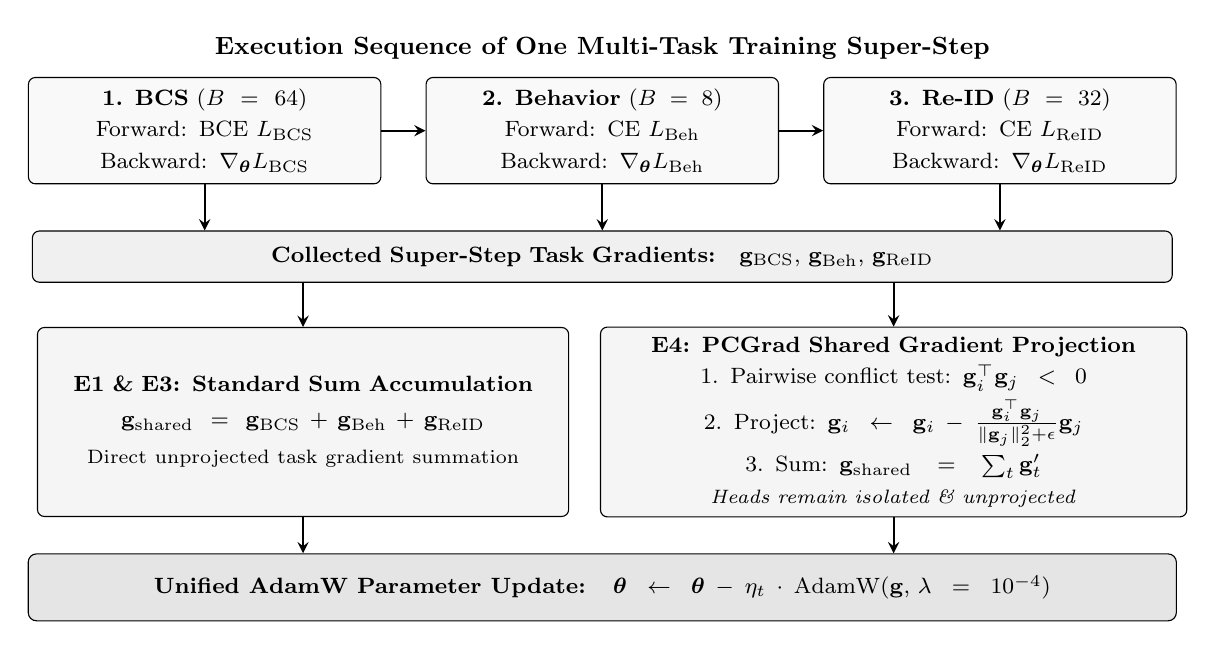
\begin{tikzpicture}[
  title/.style={font=\bfseries\small, align=center},
  stepbox/.style={draw, rectangle, rounded corners=2.5pt, align=center, font=\footnotesize, text width=4.3cm, minimum height=1.35cm, fill=gray!5, inner sep=2.5pt},
  poolbox/.style={draw, rectangle, rounded corners=2.5pt, align=center, font=\footnotesize, text width=14.3cm, minimum height=0.65cm, fill=gray!12, inner sep=2.5pt},
  branchbox/.style={draw, rectangle, rounded corners=2.5pt, align=center, font=\footnotesize, minimum height=2.40cm, fill=gray!8, inner sep=3.5pt},
  optbox/.style={draw, rectangle, rounded corners=3pt, align=center, font=\footnotesize\bfseries, text width=14.3cm, minimum height=0.85cm, fill=gray!20, inner sep=4pt},
  arrow/.style={->, >=stealth, thick}
]

\node[title] at (7.45, 1.05) {Execution Sequence of One Multi-Task Training Super-Step};

\node[stepbox] (s1) at (2.40, 0.0) {\textbf{1. BCS} ($B=64$)\\[2pt]Forward: BCE $L_{\mathrm{BCS}}$\\[2pt]Backward: $\nabla_{\boldsymbol{\theta}} L_{\mathrm{BCS}}$};
\node[stepbox] (s2) at (7.45, 0.0) {\textbf{2. Behavior} ($B=8$)\\[2pt]Forward: CE $L_{\mathrm{Beh}}$\\[2pt]Backward: $\nabla_{\boldsymbol{\theta}} L_{\mathrm{Beh}}$};
\node[stepbox] (s3) at (12.50, 0.0) {\textbf{3. Re-ID} ($B=32$)\\[2pt]Forward: CE $L_{\mathrm{ReID}}$\\[2pt]Backward: $\nabla_{\boldsymbol{\theta}} L_{\mathrm{ReID}}$};

\draw[arrow] (s1) -- (s2);
\draw[arrow] (s2) -- (s3);

\node[poolbox] (pool) at (7.45, -1.60) {\textbf{Collected Super-Step Task Gradients:}\quad $\mathbf{g}_{\mathrm{BCS}},\,\mathbf{g}_{\mathrm{Beh}},\,\mathbf{g}_{\mathrm{ReID}}$};

\draw[arrow] (s1.south) -- (s1.south |- pool.north);
\draw[arrow] (s2.south) -- (s2.south |- pool.north);
\draw[arrow] (s3.south) -- (s3.south |- pool.north);

\node[branchbox, text width=6.5cm] (branch_std) at (3.65, -3.70) {%
  \textbf{E1 \& E3: Standard Sum Accumulation}\\[3pt]
  $\mathbf{g}_{\mathrm{shared}} = \mathbf{g}_{\mathrm{BCS}} + \mathbf{g}_{\mathrm{Beh}} + \mathbf{g}_{\mathrm{ReID}}$\\[4pt]
  {\scriptsize Direct unprojected task gradient summation}
};

\node[branchbox, text width=7.2cm] (branch_pcgrad) at (11.15, -3.70) {%
  \textbf{E4: PCGrad Shared Gradient Projection}\\[2pt]
  1. Pairwise conflict test: $\mathbf{g}_i^\top \mathbf{g}_j < 0$\\[2pt]
  2. Project: $\mathbf{g}_i \leftarrow \mathbf{g}_i - \frac{\mathbf{g}_i^\top \mathbf{g}_j}{\lVert\mathbf{g}_j\rVert_2^2 + \epsilon}\mathbf{g}_j$\\[2pt]
  3. Sum: $\mathbf{g}_{\mathrm{shared}} = \sum_t \mathbf{g}'_t$\\[2pt]
  {\scriptsize \textit{Heads remain isolated \& unprojected}}
};

\draw[arrow] (branch_std.north |- pool.south) -- (branch_std.north);
\draw[arrow] (branch_pcgrad.north |- pool.south) -- (branch_pcgrad.north);

\node[optbox] (opt) at (7.45, -5.80) {Unified AdamW Parameter Update:\quad $\boldsymbol{\theta} \leftarrow \boldsymbol{\theta} - \eta_t \cdot \operatorname{AdamW}(\mathbf{g},\, \lambda=10^{-4})$};

\draw[arrow] (branch_std.south) -- (branch_std.south |- opt.north);
\draw[arrow] (branch_pcgrad.south) -- (branch_pcgrad.south |- opt.north);

\end{tikzpicture}
\end{document}